\documentclass[twocolumn, 10pt]{article}
%\usepackage[english]{babel}
%\usepackage{amsmath, amssymb, amsfonts, bm}
%\usepackage{graphicx}
%\usepackage{geometry}
%\usepackage{cite}
%\usepackage[hidelinks]{hyperref}
\setlength{\emergencystretch}{2em}
%\usepackage{booktabs}
%\usepackage{titlesec}

% REVTeX is not available in the current LaTeX installation; use the
% standard article class instead.
\usepackage[utf8]{inputenc}
\usepackage{amsmath, amsfonts, amssymb, graphicx, booktabs, xcolor, lipsum}
\usepackage[hidelinks]{hyperref}
\renewcommand{\topfraction}{0.90}
\renewcommand{\bottomfraction}{0.85}
\renewcommand{\textfraction}{0.08}
\renewcommand{\floatpagefraction}{0.75}
\renewcommand{\dbltopfraction}{0.90}
\makeatletter
\setlength{\@fptop}{0pt}
\setlength{\@dblfptop}{0pt}
\makeatother

\begin{document}

%\geometry{margin=1.7cm, top=2cm, bottom=2cm}
%\titleformat{\section}{\large\bfseries}{\thesection}{1em}{}

\title{\textbf{Mechanical Reorganization and Tracer Retention in Layered Platelet--Fibrin Networks}}

\author{Juan P. Staforelli-Vivanco$^1$, Paolo Teppa Gutierrez$^{1,*}$ \\
\small $^1$ Departamento de Física, Facultad de Ciencias Físicas y Matemáticas, \\
\small Universidad de Concepción, Concepción, Chile \\
\small $^*$ pteppa2018@udec.cl}

\date{\today}

\twocolumn[
\begin{@twocolumnfalse}
\maketitle
\vspace{-1.5em}
\begin{center}
\begin{minipage}{0.88\textwidth}
\small
\noindent
How does mechanical reorganization of a platelet--fibrin network affect finite-time particle retention? We study nine paired mechanical seed groups at four filopodial baselines, using independently generated planes assembled into 50-layer domains of fixed thickness $5~\mu\mathrm m$. Frozen states at 0, 5, 10, and 15 s are probed with 256 centrally released, noninteracting tracers per unique geometry (diameter $0.50~\mu\mathrm m$), reflecting at continuous solids and escaping through either axial face. The 29952 unique histories are observed for up to 100 s. Relative to the same-time zero-baseline control, all 81 active-baseline contrasts show greater common-domain contraction and accessible-center fraction; absolute accessible volume increases by 9.29--27.58\%. Nevertheless, restricted mean exit-time changes differ between mechanical realizations. At the 15 s mechanical state, mean survival decreases from 27.34\% to 14.32\% between the lowest and highest baselines, but this aggregate ordering does not establish a general dose response. Independent connectivity checks distinguish censored tracers with certified exit routes from six certified disconnected state-specific starts, while leaving 9894 starts unresolved. Temporal refinement in three states supports the selected step under a revised, post-analysis survival tolerance of $\pm2.5$ percentage points and a $\pm3\%$ RMST tolerance; the original $\pm2$-point criterion remains inconclusive in one state. The study provides a reproducible exploratory comparison of contraction, accessibility, and retention without interpreting finite-time survival as irreversible capture.
\end{minipage}
\end{center}
\vspace{1em}
\end{@twocolumnfalse}
]

\section{Introduction}
Platelet traction reorganizes fibrin networks, changing their projected extent and local architecture \cite{Michael2023,Prakhya2022}. Area contraction alone, however, does not determine whether a finite-size particle can move through the remaining void or reach an external boundary. Local clearance, connectivity, and the time required to traverse a connected route describe different aspects of confinement. First-passage theory provides the relevant transport observables: survival before a specified exit and the distribution of exit times \cite{Redner2001}.

The scientific question is therefore: \emph{how does mechanical reorganization change central-release retention, and are those changes associated with accessible volume, connectivity to an exit, or slower motion within connected space?} We use independently generated two-dimensional platelet--fibrin layers as an approximate three-dimensional transport domain. Tracers start internally and escape through either external $z$ face; boundary injection and binding are not included.

The comparison links projected area contraction, particle-center accessibility, the connectivity of actual starting centers, survival $S(t)$, and restricted mean first-passage time (RMST) on matched frozen snapshots. We distinguish reproducible implementation checks from unresolved discretization uncertainty and from external structural or mechanical validation. The available nine-replica force sweep is treated as a descriptive pilot, not as evidence for a universal biological force--escape relationship.

\section{Numerical Methodology}

\subsection{Overdamped Network and Platelet Dynamics}
Both fibrin nodes and platelet centers are advanced with an overdamped Langevin update. For an object $i$ with position $\mathbf q_i$, drag coefficient $\zeta_i$, total force $\mathbf F_i$, and diffusion coefficient $D_i=k_BT/\zeta_i$,
\begin{equation}
\mathbf q_i(t+\delta t)=\mathbf q_i(t)
+\frac{\delta t}{\zeta_i}\mathbf F_i(t)
+\sqrt{2D_i\delta t}\,\boldsymbol\xi_i,
\label{eq:overdamped}
\end{equation}
where $\boldsymbol\xi_i\sim\mathcal N(\mathbf 0,\mathbf I_2)$ is independently sampled for every object and coordinate. Mechanical quantities are expressed consistently in $\mu\mathrm{m}$, nN, and s. The effective drag coefficients used in the simulations are
\begin{equation}
\zeta_n=3.77\;\mathrm{nN\,s\,\mu m^{-1}},
\qquad
\zeta_p=85.2\;\mathrm{nN\,s\,\mu m^{-1}},
\end{equation}
for fibrin nodes and platelets, respectively, with $D_n=k_BT/\zeta_n$ and $D_p=k_BT/\zeta_p$. These are effective model drags: the numerical coefficients are retained from the source implementation \cite{MichaelCodeOcean2023}, but are interpreted in $\mathrm{nN\,s/\mu m}$. They are approximately $10^6$ times the Stokes estimates obtained from the viscosity and radii reported by Michael et al.~\cite{Michael2023} after conversion to these units. Their effective interpretation has not been calibrated to contraction kinetics in the present planar model; mechanical time is therefore a model time, not a validated mapping to biological contraction time.

The nodal force contains backbone and cohesive WLC forces, rest-angle bending, platelet--fibrin contact, and filopodial traction. The platelet force contains platelet--platelet interaction and the equal-and-opposite reactions to platelet--fibrin contact and filopodial traction. After each stochastic update, the common translational displacement of all free objects is removed to suppress whole-clot Brownian drift.

Forces are recomputed during adaptive internal substeps. If $v_{\max}=\max_i\|\mathbf F_i\|/\zeta_i$, the deterministic displacement criterion gives
\begin{equation}
\delta t=\min\!\left(\Delta t_{\mathrm{rem}},
\frac{\delta x_{\mathrm{target}}}{v_{\max}}\right),
\qquad
\delta x_{\mathrm{target}}=0.01\;\mu\mathrm{m}.
\label{eq:adaptive-time}
\end{equation}
Here, $\Delta t_{\mathrm{rem}}$ is the portion of the prescribed outer time step that remains to be integrated after the preceding internal substeps.
An internal step is accepted in full when its displacement remains within the numerical safety bound; a proposed displacement greater than $1\;\mu\mathrm{m}$ terminates the simulation with a diagnostic error.

\begin{figure}[t]
    \centering
    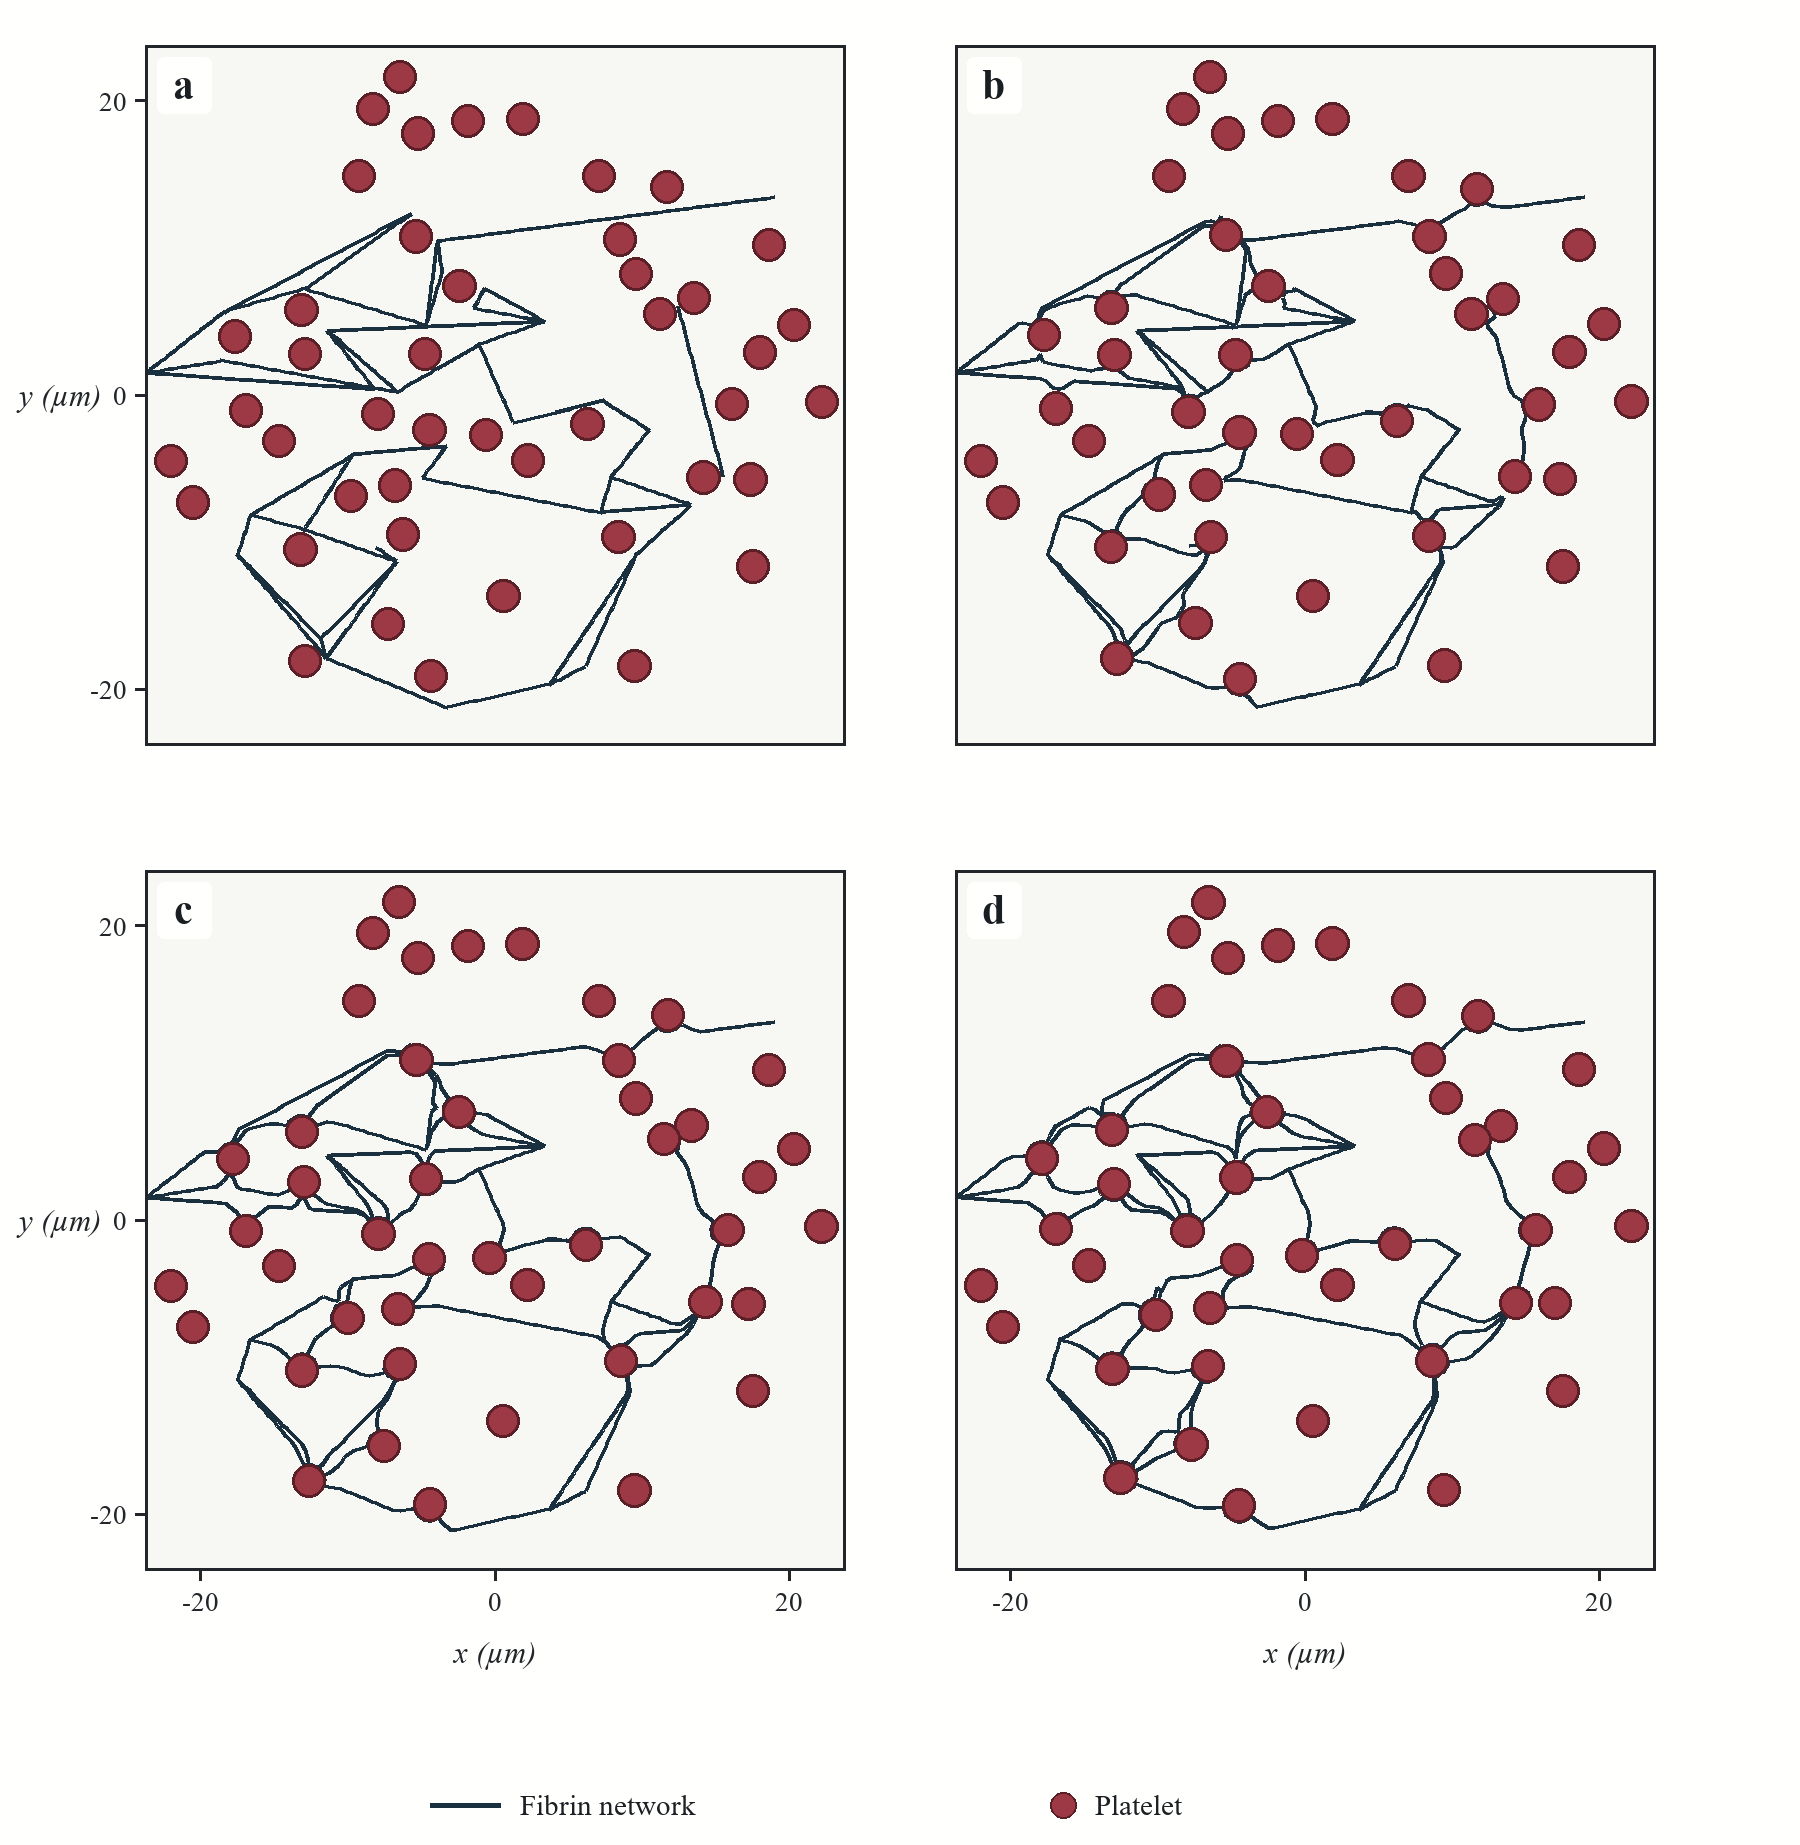
\includegraphics[width=\linewidth]{figures/figura1.png}
    \caption{Mechanical evolution of layer 1 from replica 1 of the analyzed cohort (seed 4000, $f_0=2.2\,\mathrm{nN}$) at (a) 0, (b) 2, (c) 5, and (d) 10 s. Disks denote platelets; lines denote fibrin backbone and cohesive connections. All panels use identical spatial limits and scale.}
    \label{fig1}
\end{figure}
%\subsection{DRAFT}
%Adaptive Fibrin Discretization ---  add hand-over - bending eqs. dig for $k$ used in bending (supplementary notes: energy to force $F^{bend}$)\par
%Interactions ---  add schematic or refine description of zones

%-------------------------------------------------------------------------------------------------------------%

\subsection{Initial Length-Controlled Fibrin Discretization}

Each fibrin edge is subdivided once, during construction of the initial mechanical network. For an initial edge of length $L$, the number of sub-segments $S_{\mathrm{sub}}$ is determined by the target segment length $l_{\mathrm{seg}}=0.30\;\mu\mathrm{m}$:
\begin{equation}
S_{\mathrm{sub}}=\max\!\left(2,
\left\lceil\frac{L}{l_{\mathrm{seg}}}\right\rceil\right).
\label{eq:initial-discretization}
\end{equation}
Each resulting sub-segment $e$ stores its initial length as the reference length $L_{0,e}$. Its mechanical state is described by the engineering strain
\begin{equation}
\begin{aligned}
    \gamma_e &= \frac{L_e-L_{0,e}}{L_{0,e}},
    &\widehat{\gamma}_e &= \min(\gamma_e,\gamma_{\max}),\\
    u_e &= \frac{\widehat{\gamma}_e}{C}.
\end{aligned}
    \label{eq:wlcstrain}
\end{equation}
where $C$ is a dimensionless WLC extension parameter and $0<\gamma_{\max}<C$. The WLC singularity occurs at $\gamma=C$, equivalently at $L=(1+C)L_0$. The cap $\widehat\gamma$ is used only in the constitutive evaluation, while the node coordinates evolve according to Eq.~\eqref{eq:overdamped}.

Internal stretching is governed by the Marko--Siggia WLC interpolation \cite{MarkoSiggia1995,Michael2023}. For a sub-segment representing $N$ load-bearing chains in parallel, the signed axial force is
\begin{equation}
    F_{\mathrm{WLC},e}
    = \frac{N k_B T}{P}
    \left[
        \frac{1}{4\bigl(1-u_e\bigr)^2}-\frac{1}{4}+u_e
    \right],
    \label{eq:wlcforce}
\end{equation}
where $P$ is the persistence length. Equation~\eqref{eq:wlcforce} gives $F_{\mathrm{WLC}}=0$ at the reference configuration ($\gamma=0$), positive tension under extension, and a signed compressive response for $\gamma<0$. The analytical tangent of the uncapped law, evaluated at $\widehat{\gamma}_e$, is
\begin{equation}
    k_{\gamma,e}
    = \left.\frac{\partial F_{\mathrm{WLC}}}{\partial\gamma}\right|_{\widehat{\gamma}_e}
    = \frac{N k_B T}{P}
    \left[
        \frac{C^2}{2\bigl(C-\widehat{\gamma}_e\bigr)^3}+\frac{1}{C}
    \right].
    \label{eq:wlctangent}
\end{equation}
Because $\gamma$ is dimensionless, $k_{\gamma,e}$ has units of force. A spatial spring stiffness is $k_{L,e}=k_{\gamma,e}/L_{0,e}$, with units of force per length. The stiffness signal used by a platelet attached to node $j$ is evaluated at the mean signed strain of the $n_j$ incident backbone segments,
\begin{equation}
    \overline{\gamma}_j
    = \frac{1}{n_j}\sum_{e\in S(j)}\gamma_e,
    \qquad
    k_j = k_\gamma\!\left(\min(\overline{\gamma}_j,\gamma_{\max})\right).
    \label{eq:wlcstiffness}
\end{equation}
This tangent provides the local mechanical signal entering the filopodial traction law.
\subsection{Rest-Angle Bending}
Contour preservation is represented by an angular bending energy. For a node triplet $(i,j,k)$, define the adjacent vectors and current signed turning angle as
\begin{equation}
\mathbf u=\mathbf x_j-\mathbf x_i,\qquad
\mathbf v=\mathbf x_k-\mathbf x_j,
\end{equation}
\begin{equation}
\phi=\operatorname{atan2}\!\left(
(\mathbf u\times\mathbf v)_z,\mathbf u\cdot\mathbf v\right).
\end{equation}
The angular deviation from the stored initial angle $\phi_0$ is wrapped to $(-\pi,\pi]$,
\begin{equation}
\Delta\phi=\operatorname{atan2}\!\left[
\sin(\phi-\phi_0),\cos(\phi-\phi_0)\right].
\end{equation}
With the reference dual length
\begin{equation}
\overline L_{0,ijk}=\frac{L_{0,ij}+L_{0,jk}}{2},
\end{equation}
the bending energy and forces are
\begin{equation}
E_{ijk}^{\mathrm{bend}}=
\frac{1}{2}\frac{EI}{\overline L_{0,ijk}}(\Delta\phi)^2,
\qquad
\mathbf F_{\ell}^{\mathrm{bend}}
=-\frac{\partial E_{ijk}^{\mathrm{bend}}}{\partial\mathbf x_\ell},
\label{eq:bending-energy}
\end{equation}
where $\ell\in\{i,j,k\}$ and $EI=2.26\times10^{-3}\;\mathrm{nN\,\mu m^2}$. Consequently, the three forces sum to zero. Bending triplets are assigned both along subdivided fiber interiors and between angularly adjacent segments at network junctions.
%------------------------------------------------------------------------------------------------------------%
\subsection{Platelet-Fiber Interaction}

The platelet body is represented by a circle of radius $r_p=1.13\;\mu\mathrm{m}$. Platelet--fibrin body contact acts between a platelet center $\mathbf p_m$ and fibrin node $\mathbf x_j$. Let
\begin{equation}
\mathbf r_{mj}=\mathbf x_j-\mathbf p_m,
\qquad d_{mj}=\|\mathbf r_{mj}\|,
\qquad \widehat{\mathbf r}_{mj}=\frac{\mathbf r_{mj}}{d_{mj}},
\end{equation}
and define
\begin{equation}
r_{\mathrm{in}}=f_r r_p+r_f,
\qquad r_{\mathrm{out}}=r_p+r_f,
\end{equation}
where $f_r=0.9$ and the fiber radius is $r_f=0.05\;\mu\mathrm{m}$. The force exerted by platelet $m$ on node $j$ is the constant-magnitude radial law
\begin{equation}
\mathbf F_{j\leftarrow m}^{PF}=
\begin{cases}
+F_{PF}\widehat{\mathbf r}_{mj},
&0<d_{mj}<r_{\mathrm{in}},\\
-F_{PF}\widehat{\mathbf r}_{mj},
&r_{\mathrm{in}}\le d_{mj}\le r_{\mathrm{out}},\\
\mathbf 0,&d_{mj}>r_{\mathrm{out}},
\end{cases}
\label{eq:platelet-fibrin}
\end{equation}
with $F_{PF}=4\;\mathrm{nN}$. Thus, the inner region is repulsive and the outer contact shell is adhesive. The platelet receives the reciprocal force $-\mathbf F_{j\leftarrow m}^{PF}$.

Filopodia operate in the separate annulus $r_{\mathrm{out}}\le d_{mj}\le r_{\max}$, with $r_{\max}=2.18\;\mu\mathrm{m}$. A free arm attaches to the nearest unoccupied fibrin node in this annulus. If its node leaves the annulus, the arm is released and globally reacquires the nearest available node. Global node exclusivity prevents two filopodia from claiming the same node. Each attached arm applies its full traction magnitude and an equal-and-opposite reaction to the platelet.

The filopodial traction depends on the local WLC tangent signal in Eq.~\eqref{eq:wlcstiffness}. Its stiffness-dependent contribution approaches the finite asymptote $a/b$ as $k_j$ increases, and negative total values are excluded:
\begin{equation}
F_{\mathrm{fil}}(k_j)
= \max\!\left\{0,\frac{1}{2}\left[f_0 + \frac{a k_j}{b k_j + c}\right]\right\}.
\label{eq:wlctraction}
\end{equation}
The numerical coefficient convention for $k_j$ in nN is $a=61$ nN, $b=3.58$, and $c=132$ nN. In particular, $f_0=0$ removes only the baseline term: the stiffness-dependent traction remains. It is not an inactive-platelet or noncontractile control.

\subsection{Platelet--Platelet Interaction}
Platelet pairs interact through the derivative of a truncated 12--6 Lennard--Jones potential. The core diameter, length scale, and cutoff are
\begin{equation}
d_c=2f_r r_p,\qquad
\sigma=\frac{d_c}{2^{1/6}},\qquad
r_c=2r_p.
\end{equation}
For the separation vector $\mathbf r_{ab}=\mathbf p_b-\mathbf p_a$, $r=\|\mathbf r_{ab}\|$, and $\widehat{\mathbf r}_{ab}=\mathbf r_{ab}/r$, define
\begin{equation}
f_{PP}(r)=
\begin{cases}
\displaystyle\frac{24\epsilon}{r}
\left[2\left(\frac{\sigma}{r}\right)^{12}
-\left(\frac{\sigma}{r}\right)^6\right],&r\le r_c,\\[3mm]
0,&r>r_c.
\end{cases}
\label{eq:platelet-platelet-scalar}
\end{equation}
The reciprocal pair forces are
\begin{equation}
\mathbf F_a^{PP}=-f_{PP}(r)\widehat{\mathbf r}_{ab},
\qquad
\mathbf F_b^{PP}=-\mathbf F_a^{PP},
\label{eq:platelet-platelet}
\end{equation}
with $\epsilon=4\;\mathrm{nN\,\mu m}$. The force is repulsive for $r<d_c$, zero at $r=d_c$, and attractive for $d_c<r<r_c$. The interaction is set to zero beyond $r_c$ and retains its unshifted value immediately inside the cutoff.

\subsection{Permanent Fiber--Fiber Cohesion}
New cohesive links are searched every ten outer mechanical intervals between distinct-fiber nodes separated by no more than $r_{\mathrm{coh}}=0.10\;\mu\mathrm{m}$. Existing backbone pairs, duplicate pairs, and node pairs sharing a fiber identity are excluded. At most four new cohesive links may be assigned to a node in one search and at most four cohesive neighbors are permitted per node; backbone neighbors are not counted toward this cohesive valence.

When a link $(a,b)$ is created at time $t_b$, its reference length is
\begin{equation}
L_{0,ab}^{\mathrm{coh}}
=\|\mathbf x_b(t_b)-\mathbf x_a(t_b)\|,
\qquad
F_{\mathrm{WLC}}(t_b)=0.
\label{eq:cohesion-birth}
\end{equation}
The link is permanent and subsequently carries the same signed WLC law as a backbone segment. Only one cohesive link is allowed for each unordered node pair.

\subsection{Mechanical Parameterization and Internal Balance}
Stretching follows Eqs.~\eqref{eq:wlcstrain}--\eqref{eq:wlcforce}. For every backbone or cohesive pair, the scalar WLC force is applied along the current pair direction with equal-and-opposite nodal contributions. The parameter values are $T=300$ K, $N=50$, $P=1.07\times10^{-3}\,\mu\mathrm{m}$, $C=2.35$, and $\gamma_{\max}=2.0$. The bundle multiplier $N=50$ is a choice of the planar adaptation, not the $N=1100$ assigned to a 100 nm fiber by the source implementation \cite{MichaelCodeOcean2023}. It has not been recalibrated here. Likewise, the platelet pair energy $\epsilon=4~\mathrm{nN\,\mu m}$ is an input of the adapted contact law, rather than the $16~\mathrm{nN\,\mu m}$ coefficient in the original formulation \cite{Michael2023}.

Table~\ref{tab:parameters} collects the saved mechanical settings and the homogeneous transport protocol. These are model inputs, not values fitted to the escape measurements. Mechanical settings were checked against the saved configurations: two seed blocks assembled from 20-layer stacks and 30-layer extensions, and seven generated directly with 50 layers under the same protocol. All evolutions continue to 15 s from their saved 10 s mechanical states, retaining cohesive links, their reference lengths, and stochastic continuation state. Contraction is always referenced to the original 0 s configuration. The effective $1~\mu$m thickness used to convert junction densities into planar node counts is an initialization parameter, distinct from the transport layer thickness $H$.

\begin{table*}[tp]
\centering
\footnotesize
\setlength{\tabcolsep}{4pt}
\renewcommand{\arraystretch}{1.03}
\caption{Model parameters and frozen-state transport protocol. Values are rounded for presentation; configuration files retain the values used in computation. Counts and time steps are exact. \textit{Adapted} identifies a change of interpretation, geometry, or implementation, not a new experimental calibration.}
\label{tab:parameters}
\begin{tabular}{@{}p{0.30\textwidth}p{0.43\textwidth}p{0.22\textwidth}@{}}
\toprule
Parameter or setting & Value or rule & Source \\\midrule
\multicolumn{3}{@{}l}{\textit{Mechanical network}}\\
Domain; platelets per layer & $47.6\times47.6~\mu\mathrm m$; 45 & Adapted from \cite{Michael2023}\\
\specialrule{0.2pt}{1.5pt}{1.5pt}
Platelet and fiber radii & $r_p=1.13~\mu\mathrm m$; $r_f=0.05~\mu\mathrm m$ & \cite{Michael2023,MichaelCodeOcean2023}\\
\specialrule{0.2pt}{1.5pt}{1.5pt}
Junction densities (degree 3, 4) & $0.020$, $0.00379~\mu\mathrm m^{-3}$; initialization thickness $1~\mu\mathrm m$ & This study\\
\specialrule{0.2pt}{1.5pt}{1.5pt}
Segment length; temperature & $l_{\mathrm{seg}}=0.30~\mu\mathrm m$; $T=300$ K & \cite{MichaelCodeOcean2023}\\
\specialrule{0.2pt}{1.5pt}{1.5pt}
Parallel WLC chains; strain cap & $N=50$; $\gamma_{\max}=2$ & This study\\
\specialrule{0.2pt}{1.5pt}{1.5pt}
WLC persistence and extension & $P=1.07$ nm; $C=2.35$ & \cite{MichaelCodeOcean2023}\\
\specialrule{0.2pt}{1.5pt}{1.5pt}
Bending rigidity & $EI=2.26\times10^{-3}~\mathrm{nN\,\mu m^2}$ & Adapted from \cite{Michael2023,MichaelCodeOcean2023}\\
\specialrule{0.2pt}{1.5pt}{1.5pt}
Effective node and platelet drag & $\zeta_n=3.77$, $\zeta_p=85.2~\mathrm{nN\,s/\mu m}$ & Adapted from \cite{MichaelCodeOcean2023}; see text\\
\specialrule{0.2pt}{1.5pt}{1.5pt}
Cohesive distance & $r_{\mathrm{coh}}=0.10~\mu\mathrm m$ & \cite{Michael2023,MichaelCodeOcean2023}\\
\specialrule{0.2pt}{1.5pt}{1.5pt}
Cohesive search and valence & Every 10 outer steps; at most 4 new links and 4 cohesive neighbors per node & This study\\
\specialrule{0.2pt}{1.5pt}{1.5pt}
Platelet--fibrin force & $F_{PF}=4$ nN & Magnitude: \cite{Michael2023}; law adapted\\
\specialrule{0.2pt}{1.5pt}{1.5pt}
Platelet pair energy & $\epsilon=4~\mathrm{nN\,\mu m}$ & This study\\
\specialrule{0.2pt}{1.5pt}{1.5pt}
Core fraction; filopodial reach & $f_r=0.9$; $r_{\max}=2.18~\mu\mathrm m$ & \cite{MichaelCodeOcean2023}\\
\specialrule{0.2pt}{1.5pt}{1.5pt}
Filopodial baseline sweep & $f_0\in\{0,2.2,4.4,8.8\}$ nN & This study; baseline scale \cite{Michael2023}\\
\specialrule{0.2pt}{1.5pt}{1.5pt}
Stiffness-response coefficients & $a=61$ nN, $b=3.58$, $c=132$ nN & Adapted from \cite{MichaelCodeOcean2023}\\
\specialrule{0.2pt}{1.5pt}{1.5pt}
Filopodia per platelet & Log-space $\mu=1.85$, $\sigma=0.27$; rounded and clipped to 2--13 & Distribution: \cite{Michael2023}; sampling adapted\\
\specialrule{0.2pt}{1.5pt}{1.5pt}
Mechanical integration; output & Outer step 1 ms; target displacement $0.01~\mu\mathrm m$; output every 0.1 s, up to 15 s & This study\\
\specialrule{0.2pt}{1.5pt}{1.5pt}
Lateral support & Convex support, padding $0.50~\mu\mathrm m$; $256\times256$ raster & This study\\
\midrule
\multicolumn{3}{@{}l}{\textit{Frozen-state transport and sampling}}\\
Layers and thickness & $N_z=50$; $H=100$ nm; $L_z=5~\mu\mathrm m$ & This study\\
\specialrule{0.2pt}{1.5pt}{1.5pt}
Mechanical replicas and states & 9 paired seed groups; $t_m=0$, 5, 10, 15 s & This study\\
\specialrule{0.2pt}{1.5pt}{1.5pt}
Tracer radius & $a_{\rm tr}=0.25~\mu\mathrm m$ & Chosen; size scale \cite{Zubairova2015}\\
\specialrule{0.2pt}{1.5pt}{1.5pt}
Tracer diffusion & $D=0.40~\mu\mathrm m^2/\mathrm s$ & Assumed effective value\\
\specialrule{0.2pt}{1.5pt}{1.5pt}
Central release & Cylinder radius $1.19~\mu\mathrm m$; $z\in[2,3]~\mu\mathrm m$; valid-center conditioning & This study\\
\specialrule{0.2pt}{1.5pt}{1.5pt}
Histories & 256 per unique geometry; 117 geometries, 29952 histories & This study\\
\specialrule{0.2pt}{1.5pt}{1.5pt}
Time step; observation horizon & $\Delta t=0.015625$ ms; $T_c=100$ s & This study; Supplement S8\\
\specialrule{0.2pt}{1.5pt}{1.5pt}
Solids and boundaries & Continuous extruded solids; solid/lateral reflection; both $z$ faces absorbing & This study\\
\specialrule{0.2pt}{1.5pt}{1.5pt}
Geometry proposals & 131072 shared uniform-box proposals per replica & This study\\
\specialrule{0.2pt}{1.5pt}{1.5pt}
Connectivity auxiliary grid & $512\times512\times100$; $h_{xy}\approx93.0$ nm; $h_z=50$ nm & This study; Supplement S8\\
\bottomrule
\end{tabular}
\end{table*}

\subsection{Continuous Solids and the Common Analyzed Domain}
For mechanical time $t_m$, let $A_k(t_m)$ be the padded analyzed interior of layer $k$. The lateral domain is their intersection, not the intersection of their voids:
\begin{equation}
A_\cap(t_m)=\bigcap_{k=1}^{N_z}A_k(t_m),\qquad
\mathcal A=A_\cap\times[0,L_z].
\label{eq:common-domain}
\end{equation}
Each backbone and cohesive segment is represented by a planar capsule of radius $r_f$, and each platelet by a disk of radius $r_p$. These primitives are extruded over the corresponding layer slab; their union is the solid $\mathcal S$. Cohesive links have the same geometric radius as backbone segments. The construction approximates a multilayer material; it does not impose mechanical coupling between planes or reconstruct spherical platelets and curved fibers in three dimensions.

The common lateral boundary retains the native $256\times256$ support raster, with spacing approximately $0.186~\mu\mathrm m$. It is an artificial reflecting boundary for tracer centers and is not eroded again by the tracer radius. Solid exclusion instead uses continuous center-to-solid distance. For tracer radius $a_{\rm tr}$,
\begin{equation}
\begin{aligned}
\mathcal V&=\mathcal A\setminus\mathcal S,\\
\Omega_{\rm acc}&=\{\mathbf r\in\mathcal A:
\operatorname{dist}(\mathbf r,\mathcal S)\ge a_{\rm tr}\}.
\end{aligned}
\label{eq:accessible-centers}
\end{equation}
Finite-particle clearance applies to the internal solid. Escape is defined by the center reaching either external $z$ face, not by complete clearance of the sphere beyond that face.

\section{Configuration and Structure--Transport Observables}
Nine mechanical seed blocks generate paired force conditions $f_0=0$, 2.2, 4.4, and 8.8 nN. Each stack contains 50 independently generated planes with $H=100$ nm, giving $L_z=N_zH=5~\mu\mathrm m$. Frozen snapshots at $t_m=0$, 5, 10, and 15 s are analyzed. There are 144 condition labels but 117 unique geometries, because the four forces share the same initial state within each seed block. Figure~\ref{fig1} shows the mechanical evolution of layer 1 from replica 1 at $f_0=2.2$ nN.

Figure~\ref{fig:solid-stack-current} illustrates the assembly of independent mechanical planes into the solid stack used to define tracer exclusion. The display voxelization does not replace the continuous primitives used for transport.

\begin{figure}[tbp]
\centering
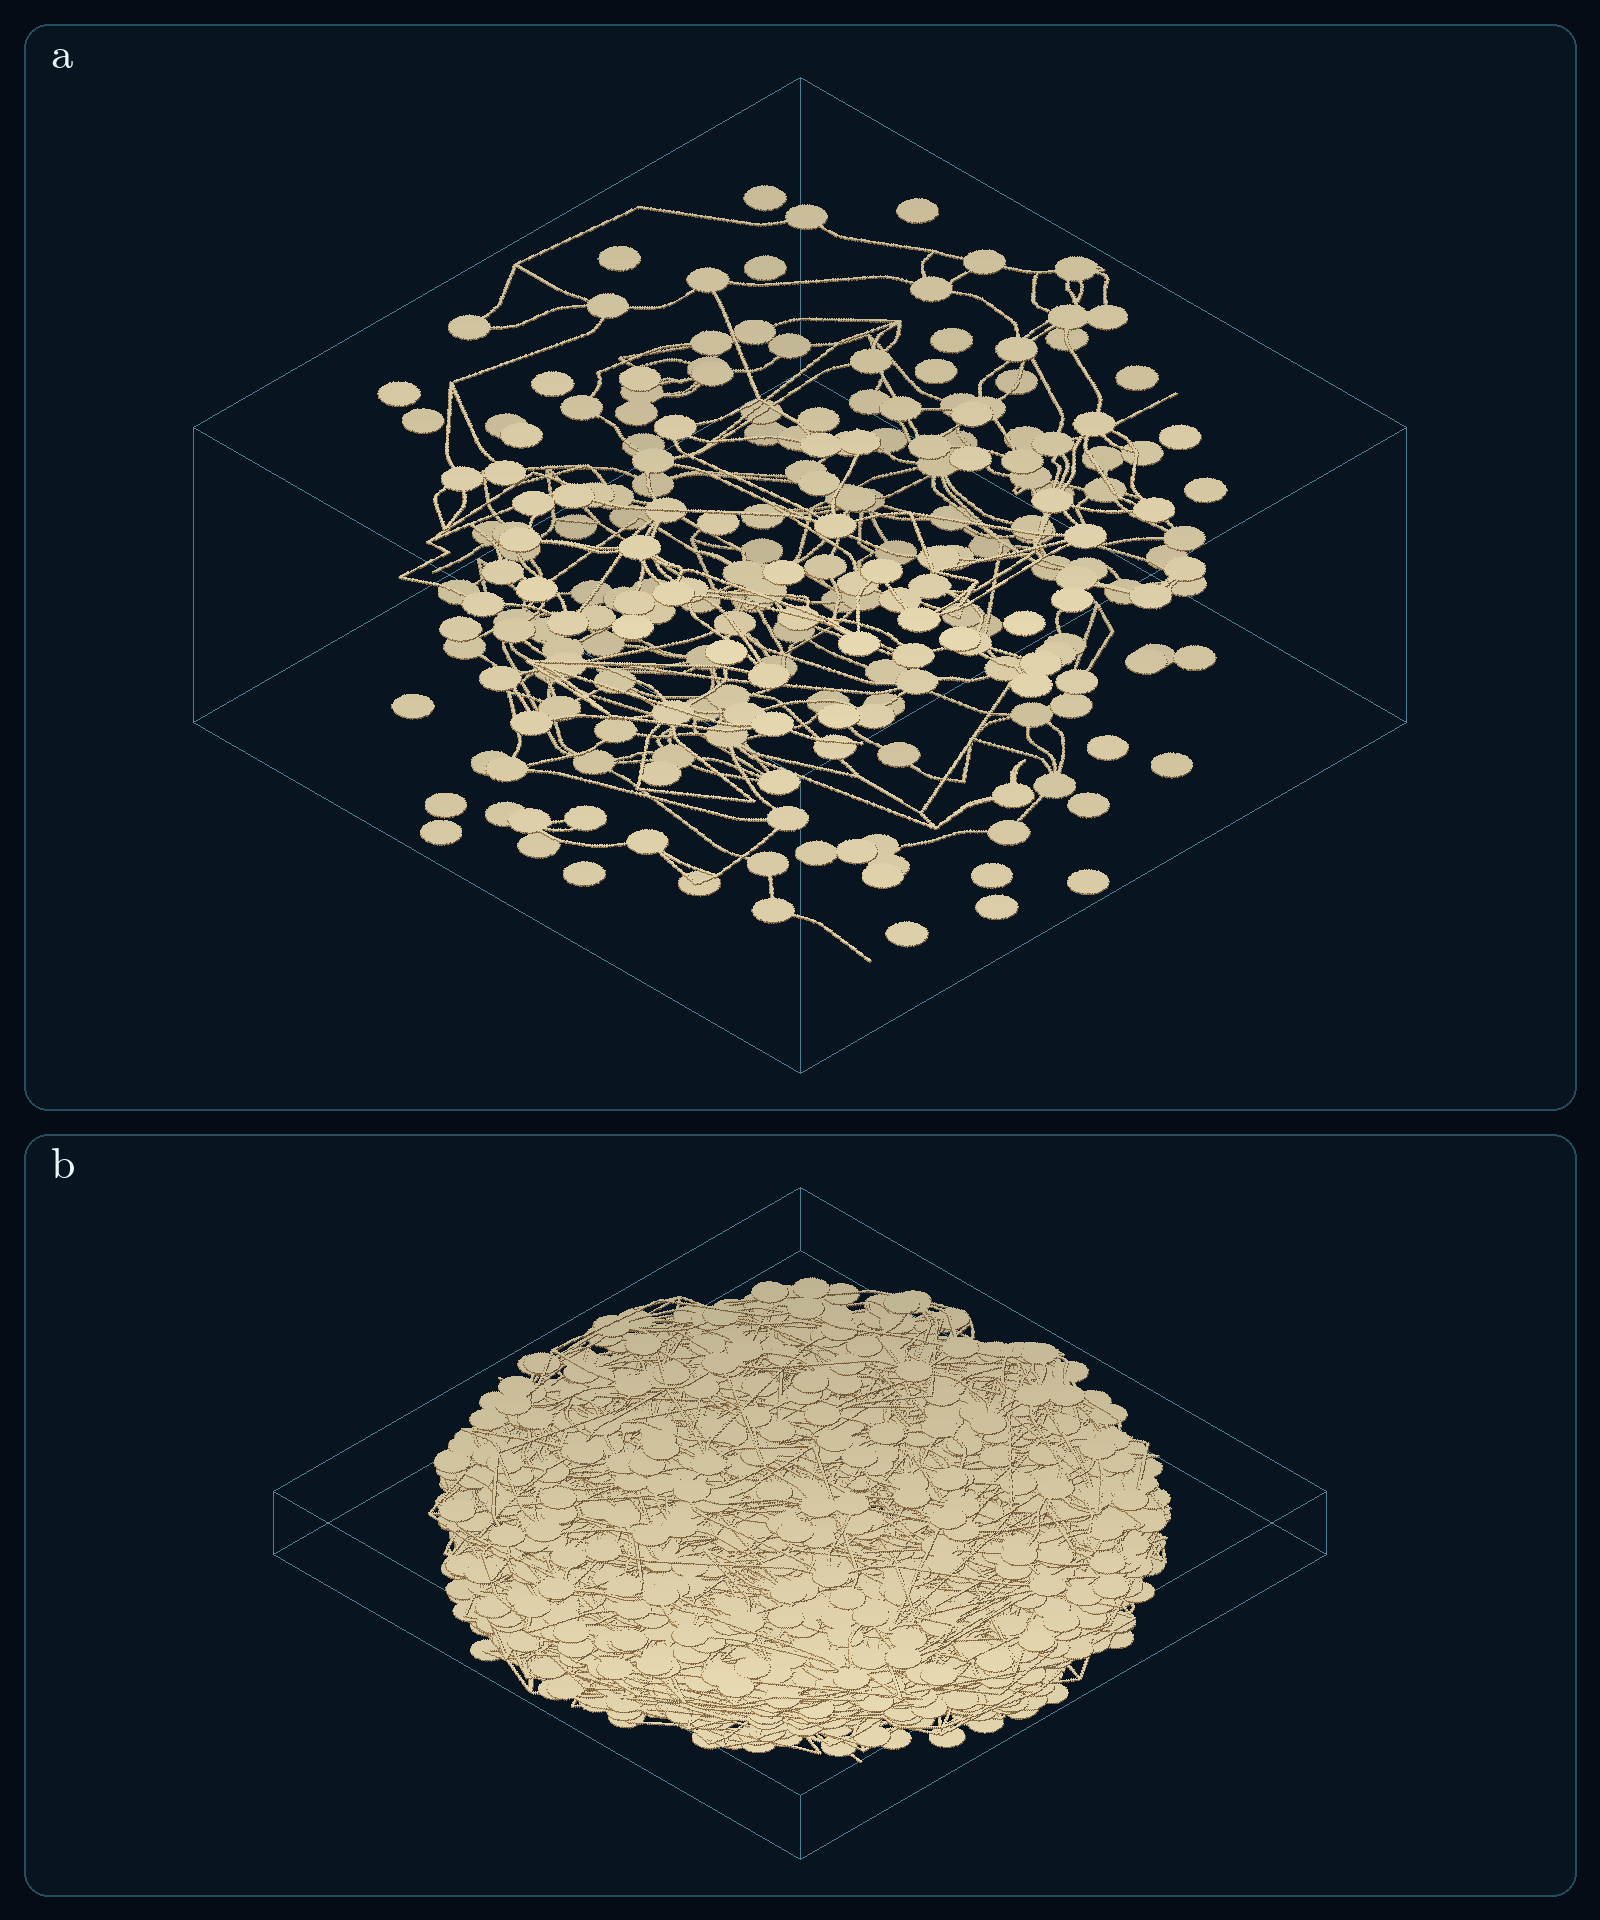
\includegraphics[width=\linewidth]{figures/figure_solid_50layer.png}
\caption{Solid assembly from replica 1 at $f_0=2.2$ nN and $t_m=10$ s. (a) Layers 1, 13, 25, 37, and 50, with separation expanded for display. (b) All 50 layers at $H=100$ nm ($L_z=5~\mu\mathrm m$), without axial exaggeration. Fibrin, cohesive links, and platelets share one opaque color. Voxels approximate the continuous solids for display only; the full lateral field is shown, without clipping to the common analyzed boundary.}
\label{fig:solid-stack-current}
\end{figure}

\subsection{Contraction, Accessibility, and Initial Connectivity}
\label{sec:structural-readouts}
Mechanical time $t_m$ selects a saved network configuration; transport time $t$ starts at tracer release and advances while that configuration remains fixed. Projected-area contraction assays motivate normalization by the initial area \cite{Prakhya2022}. We distinguish the layer-mean and common-domain measures:
\begin{equation}
\begin{aligned}
C_{A,\rm layer}(t_m)&=1-\frac{\overline{|A_k(t_m)|}}{\overline{|A_k(0)|}},\\
C_{A,\cap}(t_m)&=1-\frac{|A_\cap(t_m)|}{|A_\cap(0)|}.
\end{aligned}
\label{eq:area-contraction}
\end{equation}
Here $|A|$ denotes the area of a planar region, and $\overline{|A_k(t_m)|}=N_z^{-1}\sum_{k=1}^{N_z}|A_k(t_m)|$ is the mean area across layers.
Both characterize computationally defined projected regions, not solid-volume loss or volumetric strain. The paired results below use $C_{A,\cap}$; the layer-mean values remain in the data archive.

For the same geometry and tracer radius,
\begin{equation}
\phi_{\rm acc}=\frac{|\Omega_{\rm acc}|}{|\mathcal A|},
\qquad V_{\rm acc}=\phi_{\rm acc}|\mathcal A|.
\label{eq:accessible-fraction}
\end{equation}
Absolute accessible volume is reported alongside the fraction because contraction changes the denominator. Clearance is sampled using 131072 uniform box proposals per mechanical replica, shared across its states and restricted to the common domain. Accessibility includes valid centers in isolated components; it is not itself an escape probability.

Let $\Omega_{\rm exit}$ contain accessible centers connected to at least one absorbing $z$ face. For the $N_0$ actual starting centers, the target quantity is
\begin{equation}
\widehat F_{\rm conn}=\frac1{N_0}\sum_i
\mathbf1\{\mathbf R_i(0)\in\Omega_{\rm exit}\}.
\label{eq:initial-connectivity}
\end{equation}
Connection to both faces is unnecessary for central-release escape. Connectivity is assessed independently of the observed trajectories using conservative inner and outer cell graphs and checked continuous bridges. With $n_+$ connected, $n_-$ disconnected, and $n_?$ unresolved starts, the resulting bounds are
\begin{equation}
\frac{n_+}{N_0}\le\widehat F_{\rm conn}
\le1-\frac{n_-}{N_0}.
\label{eq:connectivity-bounds}
\end{equation}
A missing certified path does not establish isolation. Details of the auxiliary grid and bridge search are given in Supplementary Sec.~S8.

\subsection{Central Release and Reflecting Tracer Transport}
\label{sec:tracer-transport}
Each unique geometry uses 256 noninteracting spherical tracers with $a_{\rm tr}=0.25~\mu\mathrm m$ and $D=0.4~\mu\mathrm m^2\mathrm s^{-1}$. The diameter is compatible with a circulating-microparticle size scale \cite{Zubairova2015}; the diffusion coefficient is an assumed effective parameter, not measured or calibrated to that paper. Initial centers are sampled in a central cylinder of radius $1.19~\mu\mathrm m$ with $2\le z\le3~\mu\mathrm m$, conditioned on solid clearance but not exit connectivity (Fig.~\ref{fig:tracer-initialization}).

\begin{figure}[tbp]
\centering
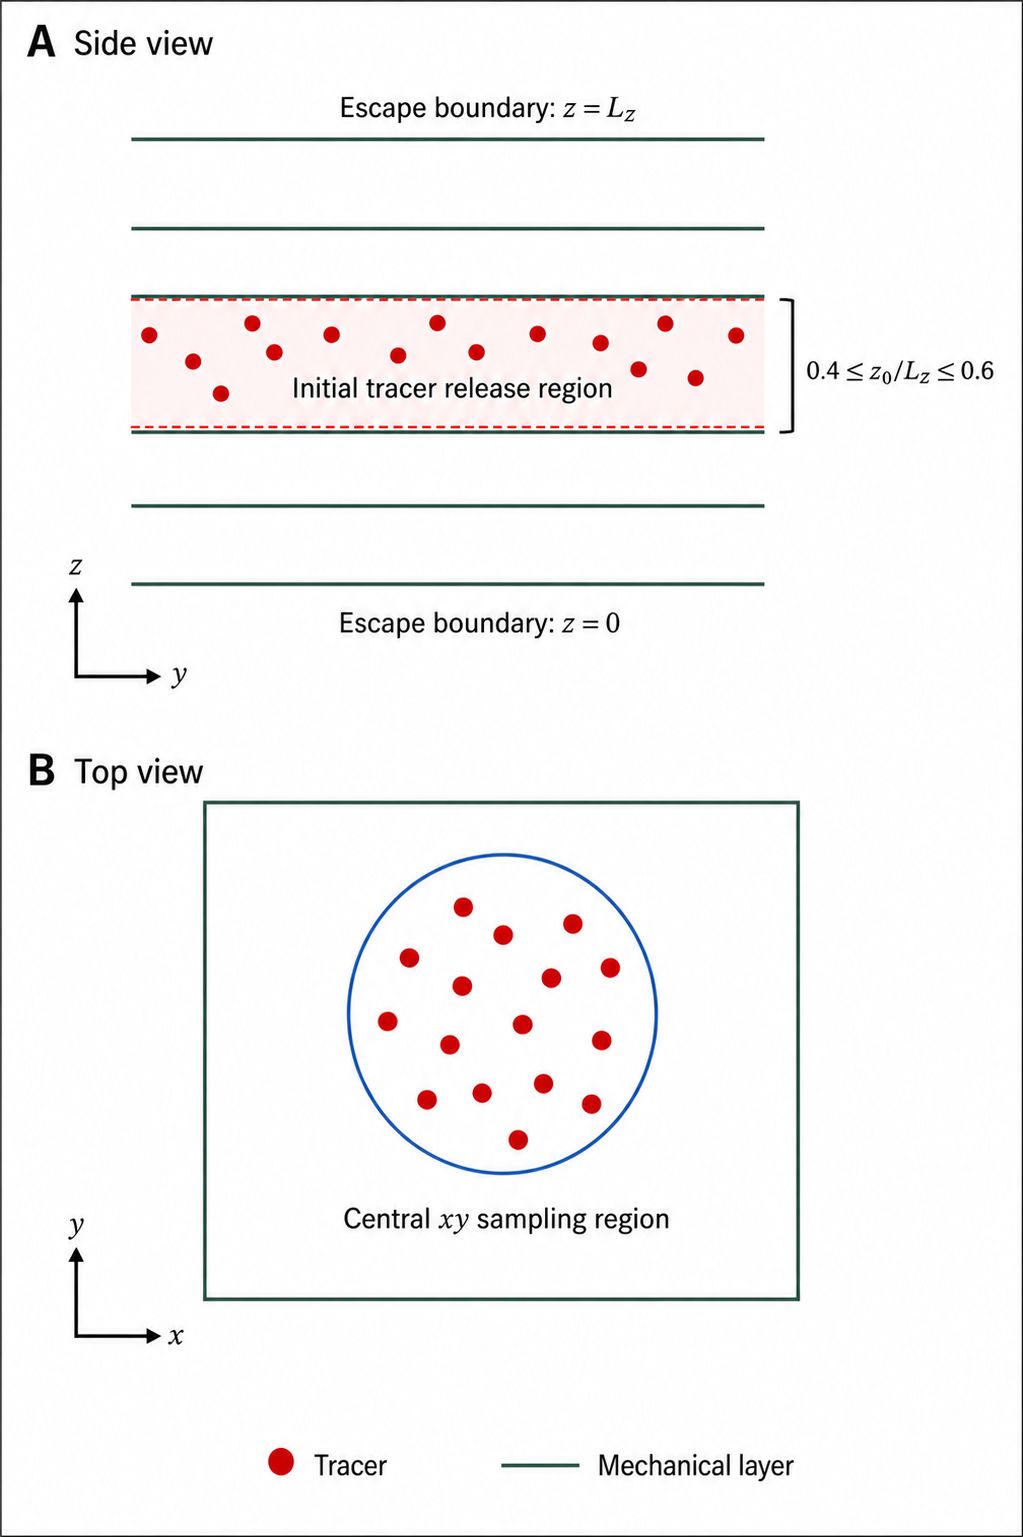
\includegraphics[width=\linewidth]{figures/tracer_initial_condition_vertical.png}
\caption{Central release in the band $0.4\le z_0/L_z\le0.6$. The lateral sampling disk has radius $1.19~\mu\mathrm m$. Escape occurs when the center first reaches $z=0$ or $z=L_z$; the analyzed lateral boundary reflects.}
\label{fig:tracer-initialization}
\end{figure}

The free proposal is
\begin{equation}
\Delta\mathbf R=\sqrt{2D\Delta t}\,\boldsymbol\eta,
\qquad\boldsymbol\eta\sim\mathcal N(\mathbf0,I_3),
\label{eq:tracer-transport}
\end{equation}
with $\Delta t=0.015625$ ms. The swept segment is checked for the first contact with the radius-expanded solid or lateral boundary. At a smooth contact with unit normal $\mathbf n$, the remaining displacement is reflected:
\begin{equation}
\Delta\mathbf R_{\rm rem}'=\Delta\mathbf R_{\rm rem}
-2(\Delta\mathbf R_{\rm rem}\cdot\mathbf n)\mathbf n.
\label{eq:reflection}
\end{equation}
Further contacts are resolved within the same increment. Simultaneous independent normals define a reflected normal subspace; a tied obstacle contact is processed before an axial exit. Geometric subdivision accommodates long sequences of reflections without resampling noise or changing physical time. Failures stop execution rather than being recorded as censoring.

This is a drift-free geometric reflection scheme, not the general force-dependent transition-probability algorithm of Behringer and Eichhorn \cite{BehringerEichhorn2012}. Its planar-wall behavior follows the image construction, whereas curved boundaries, repeated contacts, and exit timing retain finite-step error. The primary exit time is the step endpoint; a separately saved linear crossing time is not treated as an exact Brownian first-passage time.

\subsection{Survival and Restricted Mean Exit Time}
Let $\tau$ be the first time the tracer reaches either axial face. Survival is $S(t)=\Pr(\tau>t)$ \cite{Redner2001}. All histories end at escape or the common administrative horizon $T_c=100$ s, so
\begin{equation}
\widehat S(t)=1-\frac{N_{\rm escape}(t)}{N_0},
\qquad 0\le t\le T_c.
\label{eq:survival-probability}
\end{equation}
The restricted mean first-passage time is
\begin{equation}
\begin{aligned}
\widehat{\mathrm{RMST}}(T_c)
&=\frac1{N_0}\sum_i\min(\tau_i,T_c)\\
&=\int_0^{T_c}\widehat S(t)\,\mathrm dt.
\end{aligned}
\label{eq:restricted-met}
\end{equation}
Each censored history contributes $T_c$; averaging only escaped histories would estimate a different, selected quantity. The general restricted-time definition \cite{RoystonParmar2013} requires no clinical hazard model here. Finite-time survival does not demonstrate adhesion or permanent capture.

For a fixed domain and a fully resolved initial connected fraction $F_{\rm conn}$, partitioning the initial population gives
\begin{equation}
S(t)=1-F_{\rm conn}+F_{\rm conn}S_{\rm conn}(t),
\label{eq:survival-connectivity}
\end{equation}
and
\begin{equation}
\begin{aligned}
\mathrm{RMST}(T_c)={}&(1-F_{\rm conn})T_c\\
&+F_{\rm conn}\mathrm{RMST}_{\rm conn}(T_c).
\end{aligned}
\label{eq:rmst-connectivity}
\end{equation}
These identities distinguish loss of routes from slow motion in connected space. They cannot be numerically decomposed using unresolved connectivity bounds as if those bounds were exact fractions.

\subsection{Paired Comparisons and Uncertainty}
\label{sec:comparison-framework}
For an observable $Y$, each active-baseline state is compared with its own zero-baseline control at the same mechanical time:
\begin{equation}
\Delta Y_r(f_0,t_m)=Y_r(f_0,t_m)-Y_r(0,t_m).
\label{eq:paired-change}
\end{equation}
Here $r$ identifies a mechanical seed block. The control retains stiffness-dependent filopodial traction, as specified by Eq.~\eqref{eq:wlctraction}; it is not an inactive-platelet condition. Changes from the initial snapshot are stored separately.

Initial proposal pools and per-particle Gaussian seeds are reused within each replica. Validity filtering changes accepted starting coordinates: force-control pairs share 26--225 of 256 physical positions, often at different indices, and at most 68 at identical indices. Thus pairing does not imply identical physical starts. The initial population is native to each geometry and is never filtered by subsequent escape.

Transport contrasts use 10000 percentile-bootstrap resamples of paired particle indices \cite{Efron1979}. The 95\% intervals are approximate, marginal, and conditional on the chosen networks and observed starting samples. They do not provide simultaneous coverage, full uncertainty propagation through initial sampling, between-network uncertainty, or numerical error bounds. Geometry and transport contrasts retain the nine mechanical replicas separately; mean survival curves are accompanied by their minimum--maximum range. No population-level significance claim is based on 256 tracers or 50 layers as if they were independent clots. Comparisons between the 15 and 10 s mechanical states use the same paired-index procedure and remain conditional on the two accepted starting samples.

\subsection{Numerical Verification and Scope}
\label{sec:verification}
Implementation checks, analytical references, and sensitivity studies answer different questions. The supplement preserves the fixed-mask and cropped continuous-geometry studies with their original boundary rules. Their conditional conclusions are not transferred to the present reflecting, cohesion-inclusive full common domain.

The reflecting implementation passed 26510 geometric and propagation cases, including analytic first contacts, independent segment--box comparisons, planar images, and multiple-reflection controls. A larger-sample temporal study compares $\Delta t=0.03125$, 0.015625, and 0.0078125 ms until $T_c=100$ s, using 8192 paired histories per step in each of three frozen states: replica 1 at 0 s, replica 1 at $f_0=2.2$ nN and 10 s, and replica 9 at $f_0=8.8$ nN and 15 s. These are three states from two mechanical seed groups. Initial positions are identical across steps within a state, and coarse Brownian increments sum the finer increments. Independent new tracer seeds distinguish these 73728 verification histories from the 29952 production histories.

For the primary comparison, 0.015625 minus 0.0078125 ms, all three relative RMST intervals meet the $\pm3\%$ tolerance. Survival differences are $0.024$, $0.806$, and $-0.049$ pp, with marginal 97.5\% intervals $[-1.398,1.447]$, $[-0.782,2.392]$, and $[-1.424,1.326]$ pp. All meet the revised operational margin of $\pm2.5$ pp. This survival margin was revised after examining the results; the originally fixed $\pm2$ pp margin remains inconclusive for the intermediate state. Thus the selected 0.015625 ms step satisfies practical equivalence under the revised criterion in the tested states, not a successful confirmation of the original criterion \cite{Lakens2017}. Neither the revision nor the refinement changes the production trajectories. The full intervals, their construction, and the initial 256-history comparison are retained in Supplement S8. This evidence does not establish uniform survival-curve equivalence, every-state temporal convergence, or spatial transport convergence.

\section{Results: Homogeneous Frozen-State Pilot}
The cohort contains nine paired mechanical seed blocks per force. Block 1 uses layer seeds 4000--4019 and 4040--4069; block 2 uses 4020--4039 and 4070--4099. Blocks 3--9 use consecutive groups of 50 seeds from 4100--4149 through 4400--4449. Each force reuses these blocks. There are 29952 unique tracer histories over 117 geometries. The cohort was extended sequentially: 13824 completed histories in blocks 1--6 at 0, 5, and 10 s were retained, and 16128 histories cover blocks 7--9 at those times and all nine blocks at 15 s. The per-state allocation of 256 histories was fixed before analyzing each batch, without outcome-dependent trajectory stopping.

\begin{table*}[t]
\centering\footnotesize
\setlength{\tabcolsep}{3.4pt}
\caption{Homogeneous frozen-state pilot. Values are means across nine paired mechanical replicas; bracketed transport ranges are minimum--maximum, not confidence intervals. Each unique geometry has 256 histories, tracer diameter $0.50~\mu\mathrm m$, $D=0.4~\mu\mathrm m^2/\mathrm s$, and $T_c=100$ s. The shared initial state is listed once. Contraction refers to the common analyzed region.}
\label{tab:homogeneous-pilot}
\begin{tabular}{@{}rrrrcc@{}}
\toprule
$t_m$ (s) & $f_0$ (nN) & $C_{A,\cap}$ (\%) & $\phi_{\rm acc}$ (\%) & $S(100)$ (\%) & RMST(100) (s) \\ \midrule
0 & all & 0.000 & 15.322 & $24.22\ [12.11,53.12]$ & $55.97\ [43.53,76.40]$ \\
\specialrule{0.2pt}{1.5pt}{1.5pt}
5 & 0 & 0.034 & 15.375 & $25.48\ [10.55,55.86]$ & $56.23\ [42.51,76.58]$ \\
\specialrule{0.2pt}{1.5pt}{1.5pt}
5 & 2.2 & 1.112 & 17.180 & $21.35\ [10.94,41.02]$ & $51.63\ [41.55,69.39]$ \\
\specialrule{0.2pt}{1.5pt}{1.5pt}
5 & 4.4 & 1.725 & 17.929 & $17.53\ [4.69,29.30]$ & $50.04\ [40.04,61.34]$ \\
\specialrule{0.2pt}{1.5pt}{1.5pt}
5 & 8.8 & 2.466 & 18.610 & $18.01\ [9.77,27.73]$ & $48.74\ [36.76,62.34]$ \\
\specialrule{0.2pt}{1.5pt}{1.5pt}
10 & 0 & 0.064 & 15.436 & $27.08\ [14.06,60.55]$ & $56.91\ [44.65,78.36]$ \\
\specialrule{0.2pt}{1.5pt}{1.5pt}
10 & 2.2 & 1.845 & 17.979 & $19.92\ [12.11,29.69]$ & $50.56\ [41.76,61.81]$ \\
\specialrule{0.2pt}{1.5pt}{1.5pt}
10 & 4.4 & 2.727 & 18.806 & $18.45\ [8.20,34.77]$ & $48.82\ [36.58,66.03]$ \\
\specialrule{0.2pt}{1.5pt}{1.5pt}
10 & 8.8 & 3.586 & 19.517 & $15.54\ [6.25,29.69]$ & $45.57\ [33.20,57.33]$ \\
\specialrule{0.2pt}{1.5pt}{1.5pt}
15 & 0 & 0.128 & 15.548 & $27.34\ [17.19,55.86]$ & $56.47\ [45.46,76.39]$ \\
\specialrule{0.2pt}{1.5pt}{1.5pt}
15 & 2.2 & 2.426 & 18.531 & $18.53\ [9.38,32.81]$ & $49.69\ [38.32,66.49]$ \\
\specialrule{0.2pt}{1.5pt}{1.5pt}
15 & 4.4 & 3.649 & 19.512 & $16.97\ [7.81,39.06]$ & $47.46\ [35.54,67.27]$ \\
\specialrule{0.2pt}{1.5pt}{1.5pt}
15 & 8.8 & 4.602 & 20.116 & $14.32\ [6.25,29.69]$ & $43.97\ [32.27,59.03]$ \\
\bottomrule
\end{tabular}
\end{table*}


\subsection{Geometric Reorganization}
Figure~\ref{fig:homogeneous-geometry} shows the geometric response of each mechanical replica at 15 s.
In all 81 active-baseline versus zero-baseline contrasts at 5, 10, and 15 s, both common-domain contraction and accessible-center fraction increased. Absolute accessible volume increased by 9.29--27.58\% relative to the matched control, so the fractional change is not merely a shrinking-denominator effect. At 15 s, mean $C_{A,\cap}$ rises from 0.128\% at $f_0=0$ to 4.602\% at 8.8 nN, while mean accessibility rises from 15.548\% to 20.116\% (Table~\ref{tab:homogeneous-pilot}). These are model-geometry estimates, not measurements of a real clot.

\begin{figure}[tbp]
\centering
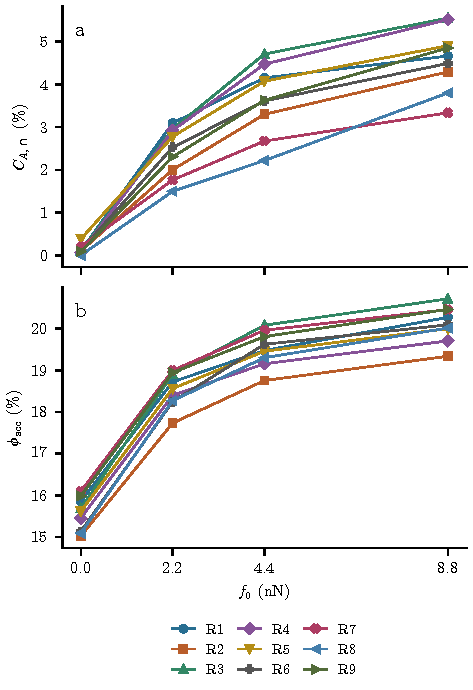
\includegraphics[width=\linewidth]{figures/homogeneous_geometry_tm15.pdf}
\caption{Frozen 15 s geometry: (a) contraction of the common analyzed area and (b) accessible-center fraction. Symbols distinguish the nine paired mechanical replicas. Lines guide the eye; no fitted dose--response law is implied.}
\label{fig:homogeneous-geometry}
\end{figure}

\subsection{Escape and Between-Realization Heterogeneity}
Figure~\ref{fig:homogeneous-transport} compares survival curves and within-replica RMST contrasts at 15 s. Replica-mean survival at 100 s decreases from 27.34\% to 14.32\% between $f_0=0$ and 8.8 nN, while RMST decreases from 56.47 to 43.97 s. Of the 27 active-control contrasts at this mechanical time, 25 have negative RMST point estimates and 21 have conditional intervals entirely below zero. At 8.8 nN, the nine within-replica reductions range from 3.59 to 20.70 s; only the interval for replica 9 includes zero. Replica 9 also has small positive point contrasts at 2.2 and 4.4 nN, and replica 6 has greater RMST at 8.8 than at 4.4 nN despite remaining below its control. The ordering of the aggregate means is therefore not a universal monotonic response.

For example, at 10 s and 4.4 nN, accessible fraction increases by 3.21 pp in replica 1 and 3.02 pp in replica 2, but the RMST changes are $+1.43$ and $-14.04$ s, respectively. Global accessibility alone therefore does not determine the observed residence time. The zero-baseline state of replica 4 at 10 s has $S(100)=60.55\%$ and RMST $=78.36$ s. This realization is retained in the means and ranges, rather than discarded as an outlier. Differences contain both network heterogeneity and conditional tracer-sampling noise; nine replicas do not by themselves establish a general force-effect claim.

\begin{figure}[tbp]
\centering
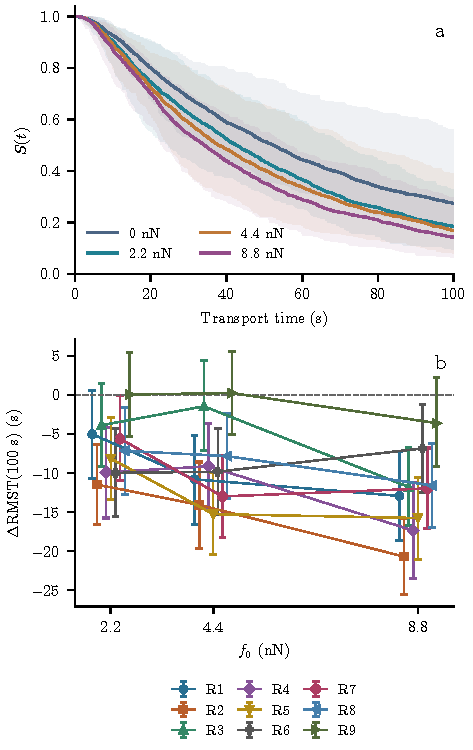
\includegraphics[width=\linewidth]{figures/homogeneous_transport_tm15.pdf}
\caption{Frozen 15 s transport. (a) Mean survival across nine replicas; shading spans their minimum--maximum range, not a confidence interval. (b) Individual-replica RMST differences from the matched $f_0=0$ control, with approximate 95\% conditional bootstrap intervals. These bars do not represent between-clot uncertainty.}
\label{fig:homogeneous-transport}
\end{figure}

Two of 29952 histories contacted the artificial lateral wall: one in replica 8 at 2.2 nN and 10 s (981 contacts), and one in replica 8 at 8.8 nN and 15 s (73 contacts). Direct lateral reflections are therefore rare at the population level, although repeated contacts can occur in an individual history. This count does not exclude effects of the domain definition on geometry or release conditioning. The absorbing-face separation remains 5 $\mu$m; rearrangement does not shorten that axial separation.

\subsection{Comparison Across Frozen Mechanical Times}
Figure~\ref{fig:homogeneous-time} separates the saved mechanical time from the subsequent 100 s transport experiment. With the same nine replicas, advancing the mechanical state from 10 to 15 s changes mean RMST by $-0.44$, $-0.87$, $-1.36$, and $-1.59$ s at baselines 0, 2.2, 4.4, and 8.8 nN, respectively. At the highest baseline, mean $S(100)$ decreases from 15.54\% to 14.32\%, while mean common-area contraction increases from 3.586\% to 4.602\%.

The modest aggregate shifts do not imply uniformly faster escape with further mechanical evolution. Among the 27 active-baseline 15-minus-10 s comparisons, only 14 have negative RMST point differences and five have conditional intervals entirely below zero. Point differences span $-9.08$ to $+4.68$ s. These are comparisons of newly released populations in two frozen geometries, not trajectories followed through a moving network.

\begin{figure}[tbp]
\centering
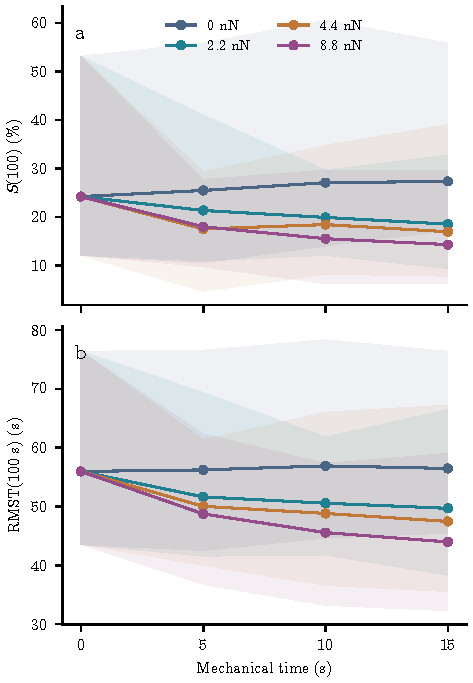
\includegraphics[width=\linewidth]{figures/homogeneous_time_evolution.pdf}
\caption{Frozen-state readouts versus mechanical time: (a) survival at 100 s and (b) RMST restricted to 100 s. Points are means over the same nine replicas; bands span their minimum--maximum range, not confidence intervals. The initial state is shared across forces.}
\label{fig:homogeneous-time}
\end{figure}

\subsection{Connectivity and Finite-Time Retention}
Independent classification certified 20052 connected starts and six disconnected state-specific starts, leaving 9894 unresolved. These are bookkeeping totals across unique conditions, not independent mechanical replicates. Of 6100 histories censored at 100 s, 3380 began at certified connected centers, six at disconnected centers, and 2714 at unresolved centers.

In replica 1 at $f_0=2.2$ nN and $t_m=10$ s, 255 of 256 starts were certified connected. All 64 censored histories belonged to that connected group: their finite-time retention cannot be attributed to an isolated compartment in the specified geometry. Conversely, replica 1 at 4.4 and 8.8 nN and 10 s left all 256 starts unresolved, despite 184 and 205 observed escapes. A zero lower connectivity bound is not zero actual connectivity.

Replica 4 contains one certified disconnected start at 4.4 nN and two at 8.8 nN at 10 s, and one at 2.2 nN and two at 4.4 nN at 15 s. None escaped by 100 s, providing a small non-vacuous consistency check. These six state-specific classifications involve two distinct starting coordinates reused across geometries, not six distinct isolated pores. The wide independent connectivity bounds do not identify the isolated fraction precisely or explain most censored histories.

\section{Discussion}
The supported finding is a separation between geometric accommodation and escape kinetics. Increasing the filopodial baseline produced more projected contraction and accessible volume in all nine seed blocks, but did not produce the same RMST response in each realization. At the highest baseline and 15 s, all nine point estimates favor lower restricted residence, while responses at lower baselines remain heterogeneous. Further evolution from 10 to 15 s yields smaller mean shifts and mixed realization-level changes. Larger accessible volume can coexist with a slowly escaping central population. Certified-connected censored histories demonstrate this distinction; the few certified disconnected starts establish that isolation also occurs in the model without showing that it dominates retention.

The comparison remains exploratory for three reasons. First, nine independent mechanical seed groups show substantial between-realization heterogeneity, and the reported conditional intervals do not establish population-level robustness. Second, the accepted initial distribution changes with geometry, so route changes are not isolated from changes in valid release positions. Third, temporal support is conditional on three tested states and a survival tolerance revised after analysis, while parts of the connectivity classification remain unresolved. Additional mechanical replicas do not themselves resolve numerical error. The revised practical acceptance does not provide numerical bounds for every state or replace external validation.

The construction uses independent mechanical planes and an imposed slab thickness, not a mechanically connected 3D reconstruction. Taking $H=100$ nm equal to the nominal fiber diameter is a modeling choice, not an experimentally established interlayer spacing. The common lateral region and reflecting convention define the analyzed domain; they should not be identified with the exterior of a biological clot. No flow, adhesion, tracer--tracer interaction, permeability, or binding kinetics is modeled. Neither a Brinkman length nor an independent aggregation rate is inferred from these escape histories. Hydraulic tortuosity concerns fluid streamlines \cite{Duda2011} and is not equated to the present restricted residence time.

The free-interval result $u(z)=z(L_z-z)/(2D)$ \cite[Chap.~2]{Redner2001} explains why prescribed thickness and initial axial position matter. A midpoint value $L_z^2/(8D)$ is a useful reference, but it is not an exact normalization for a clearance-conditioned band of starts or a censored observation. We therefore retain $S(t)$ and RMST as the primary transport readouts rather than reporting an unqualified tortuosity or a raster-dependent pore-size ratio.

\section{Conclusion and Proposed Continuation}
The completed homogeneous pilot links frozen mechanical states to finite-size accessibility, independently bounded connectivity, and censor-aware escape statistics. Within all nine mechanical seed groups, active-baseline states had greater common-domain contraction and accessibility than their matched zero-baseline controls. The highest-baseline 15 s state had a lower point estimate of restricted residence in every replica, but the size and lower-baseline direction of the effects remained realization-dependent. Advancing the frozen mechanical state from 10 to 15 s did not consistently reduce residence in individual replicas. The results support distinguishing accessible volume, availability of a route, and the time needed to follow it; they do not establish that contraction universally accelerates escape.

This stage closes as a reproducible descriptive study, with numerical and biological limits retained explicitly. Future work can add independently paired mechanical replicas, improve connectivity certification at unresolved starts, and compare transport in frozen states with transport during mechanical evolution. The last comparison requires a rule for moving-boundary encounters and must remain distinct from the present frozen experiments. Structural and mechanical comparison against the reference model or microscopy is proposed as external validation, not claimed as completed.

\paragraph{Data and supplementary material.}
The companion numerical supplement separates historical fixed-mask/local tests (S1--S7) from the current reflection checks and homogeneous analysis (S8). Tables, paired contrasts, survival horizons, trajectory counters, and source hashes for the present cohort are supplied in \path{data/homogeneous_pilot/}. Completed transport on 54 geometries was reused unchanged; 63 additional geometries contributed 252 new blocks of 64 histories. Mechanical evolutions were continued from saved states rather than restarted, and completed transport histories were not repeated.


\bibliographystyle{unsrt}
\bibliography{refs}

\end{document}
